% ============================================================================
% SEC02.TEX
% Section 1.2: Genre Game dan Karakteristiknya
% ============================================================================

\section{Genre Game dan Karakteristiknya}

\begin{learningoutcomes}
\item Mengidentifikasi berbagai genre game utama
\item Menjelaskan karakteristik setiap genre
\item Menganalisis mekanik khas dari setiap genre
\item Menerapkan pengetahuan genre dalam desain game
\end{learningoutcomes}

\subsection{Pengertian Genre Game}

\begin{definisi}[Genre Game]
Genre game adalah kategori yang mengklasifikasikan game berdasarkan mekanik gameplay, setting, atau gaya permainan yang dominan \cite{Schell2019}.
\end{definisi}

Genre membantu pemain memahami apa yang diharapkan dari sebuah game dan membantu developer mengkomunikasikan konsep game mereka.

\subsection{Genre Game Utama}

\begin{figure}[ht]
    \centering
    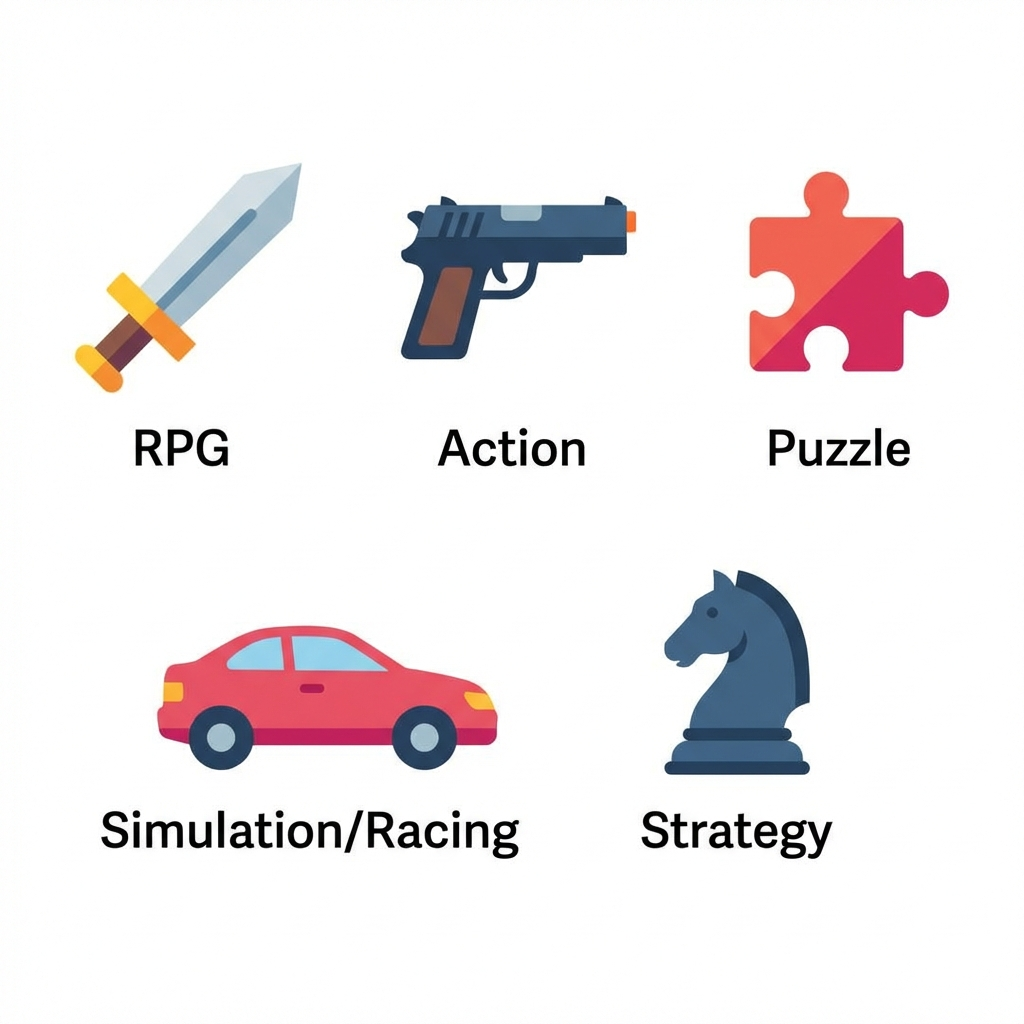
\includegraphics[width=0.8\textwidth]{figures/game_genres.png}
    \caption{Visualisasi Ikon Genre Game Utama}
    \label{fig:game_genres}
\end{figure}

\subsubsection{Action Games}

\textbf{Karakteristik}:
\begin{itemize}
\item Fokus pada refleks dan koordinasi tangan-mata
\item Gameplay cepat dan intens
\item Sering melibatkan combat atau konflik langsung
\item Contoh: Call of Duty, Devil May Cry, Dark Souls
\end{itemize}

\textbf{Sub-genre}: First-Person Shooter (FPS), Third-Person Shooter (TPS), Hack and Slash, Beat 'em up

\subsubsection{Adventure Games}

\textbf{Karakteristik}:
\begin{itemize}
\item Fokus pada narasi dan eksplorasi
\item Puzzle-solving sebagai mekanik utama
\item Interaksi dengan karakter dan lingkungan
\item Contoh: The Legend of Zelda, Uncharted, Life is Strange
\end{itemize}

\textbf{Sub-genre}: Point-and-click, Action-Adventure, Narrative Adventure

\subsubsection{Role-Playing Games (RPG)}

\textbf{Karakteristik}:
\begin{itemize}
\item Karakter development dan progression
\item Sistem statistik (HP, MP, Level, dll)
\item Quest dan mission-based gameplay
\item Contoh: Final Fantasy, The Elder Scrolls, The Witcher
\end{itemize}

\textbf{Sub-genre}: JRPG, WRPG, Action RPG, MMORPG

\subsubsection{Strategy Games}

\textbf{Karakteristik}:
\begin{itemize}
\item Fokus pada perencanaan dan taktik
\item Resource management
\item Decision-making jangka panjang
\item Contoh: Civilization, StarCraft, XCOM
\end{itemize}

\textbf{Sub-genre}: Real-Time Strategy (RTS), Turn-Based Strategy (TBS), Tower Defense

\subsubsection{Simulation Games}

\textbf{Karakteristik}:
\begin{itemize}
\item Simulasi sistem kehidupan nyata
\item Realisme dan akurasi
\item Open-ended gameplay
\item Contoh: The Sims, SimCity, Flight Simulator
\end{itemize}

\textbf{Sub-genre}: Life Simulation, City Building, Vehicle Simulation

\subsubsection{Sports Games}

\textbf{Karakteristik}:
\begin{itemize}
\item Simulasi olahraga nyata
\item Realisme dalam gameplay
\item Multiplayer competitive
\item Contoh: FIFA, NBA 2K, Madden NFL
\end{itemize}

\subsubsection{Puzzle Games}

\textbf{Karakteristik}:
\begin{itemize}
\item Fokus pada problem-solving
\item Logic-based challenges
\item Sering tidak memiliki time pressure
\item Contoh: Tetris, Portal, The Witness
\end{itemize}

\subsubsection{Platformer Games}

\textbf{Karakteristik}:
\begin{itemize}
\item Fokus pada jumping dan navigation
\item Level design dengan platform
\item Precision movement
\item Contoh: Super Mario Bros, Celeste, Hollow Knight
\end{itemize}



\begin{description}
    \item[Action] Fokus refleks, combat, tempo cepat. Contoh: CoD, Devil May Cry.
    \item[Adventure] Narasi, eksplorasi, puzzle. Contoh: Zelda, Uncharted.
    \item[RPG] Stats, progression, cerita. Contoh: Final Fantasy, Skyrim.
    \item[Strategy] Taktik, manajemen sumber daya. Contoh: Civilization, StarCraft.
    \item[Simulation] Realisme, simulasi sistem. Contoh: The Sims, Flight Sim.
    \item[Sports] Simulasi olahraga, kompetisi. Contoh: FIFA, NBA 2K.
    \item[Puzzle] Logika, pemecahan masalah. Contoh: Tetris, Portal.
    \item[Platformer] Navigasi, lompatan presisi. Contoh: Super Mario, Celeste.
\end{description}

\subsection{Hybrid Genre}

Banyak game modern menggabungkan elemen dari beberapa genre:
\begin{itemize}
\item Action-RPG: Kombinasi action combat dengan RPG progression
\item Survival Horror: Kombinasi horror dengan survival mechanics
\item Metroidvania: Kombinasi platformer dengan exploration RPG
\end{itemize}

\begin{catatan}
Genre bukanlah kategori yang kaku. Game modern sering menggabungkan elemen dari berbagai genre untuk menciptakan pengalaman yang unik.
\end{catatan}
